\section{Komunikasi Arduino Firmata}
\subsection{Firmata}
	Sebelum Arduino, domain aplikasi berbasis mikrokontroler terbatas programmer perangkat keras. Arduino membuatnya sederhana untuk pengembang yang berasal dari yang lain bidang perangkat lunak dan bahkan untuk komunitas non-coding untuk mengembangkan berbasis mikrokontroler aplikasi perangkat keras. Arduino terdiri dari desain perangkat keras sederhana dengan mikrokontroler dan I / O pin untuk antarmuka perangkat eksternal. Jika seseorang bisa menulis Arduino 
	Firmata adalah protokol umum yang memungkinkan komunikasi antara mikrokontroler dan perangkat lunak yang di-host di komputer. 
	Perangkat lunak apa pun dari host komputer apa pun yang mampu berkomunikasi serial dapat berkomunikasi dengan mikrokontroler menggunakan Firmata. 
	Firmata memberikan akses lengkap Arduino langsung ke perangkat lunak dan menghilangkan proses memodifikasi dan mengunggah sketsa Arduino. 
	Untuk memanfaatkan protokol Firmata, pengembang dapat mengunggah sketsa yang mendukung protokol ke klien Arduino sebagai proses yang dapat dilakukan sekali pakai. 
	Setelah itu, pengembang dapat menulis perangkat lunak khusus pada komputer host dan melakukan tugas-tugas kompleks. Perangkat lunak ini akan menyediakan perintah melalui port serial ke papan Arduino yang dilengkapi dengan Firmata. Dia dapat terus mengubah logika pada komputer induk tanpa mengganggu perangkat keras Arduino. 
	Praktek menulis sketsa Arduino kustom masih berlaku untuk aplikasi mandiri di mana dewan Arduino harus melakukan tugas secara lokal. Kami akan mengeksplorasi kedua opsi ini di bab-bab yang akan datang.

\subsection{Membaca Data dari Arduino ke MATLAB menggunakan Firmata}
	Firmata dapat membuat kita mengontrol arduino dengan MATLAB tanpa perlu memasukkan program khusus ke dalam arduino. Jadi firmata berfungsi sebagai penyambung agar arduino dapat berkomunikasi menggunakan bahasa pemrograman yang lain.
	
	Untuk melakukannya, berikut ini adalah langkah - langkah atau prosesnya :
		\begin{enumerate}
			\item Instalasi Pustaka Arduino.
				Saat koneksi antara MATLAB dan arduino pertama kali dibangun, disitu MATLAB mengupload pustaka dari firmata ke dalam arduino. Jadi kita harus menginstalasi nya terlebih dahulu.
			\item Koneksikan MATLAB dan Arduino.
				Sesudah menginstalasi pustaka tersebut telah selesai, hubungkan Arduino dan MATLAB menggunakan kabel serial USB. Lalu, check PORT yang Arduino gunakan untuk berhubungan ato berkomunikasi dengan MATLAB. Langkah ini dapat kita cari di dalam Device Manager jika kita menggunakan sistem operasi windows, setelah itu carilah di section PORT(COM&LPT), seperti yang di tunjukkan pada gambar dibawah ini.
				
				\begin{figure}[ht]
					\centerline{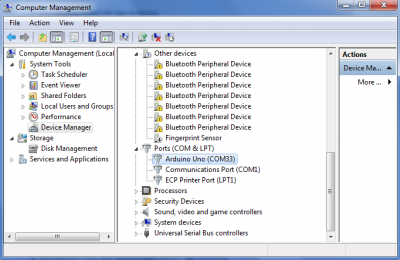
\includegraphics[width=0.5\textwidth]{figures/knksi.png}}
					\caption{Cari PORT yang dipakai Arduino}
					\label{knksi}
			\end{figure}
				
				Setelah itu, ketikkanlah sintaks atau script ini di Command Window dari MATLAB :
				
				\begin{verbatim}
				>> a = arduino
				\end{verbatim}	
				
				Setelah kita menunggu sebentar, MATLAB akan Memberikan respon seperti ini :
				
				\begin{verbatim}
				a = 
 
					arduino with properties:
 
								Port: 'COM33'
								Board: 'Uno'
							AvailableAnalogPins: [0, 1, 2, 3, 4, 5]
						AvailableDigitalPins: [2, 3, 4, 5, 6, 7, 8, 9, 10, 11, 12, 13]
							Libraries: {'I2C', 'SPI', 'Servo'}
				\end{verbatim}
				
				Berdasarkan keterangan yang dipaparkan diatas, dapat kita lihat bahwa jenis arduino yang sedang kita gunakan adalah Arduino UNO, dengan port nya yaitu COM33. Semua pin dan pustaka yang tersedia pun ditampilkan juga di layar. Jangan heran jika komputer anda menunjukkan hasil keterangan yang berbeda, karen semua tergantung jenis papan Arduino anda dan PORT atau COM yang kalian gunakan.